\documentclass{article}
\usepackage[utf8]{inputenc}
\usepackage[T5]{fontenc}
\usepackage{graphicx}
\usepackage[margin=2cm]{geometry}
\title{Report 3: Hello, CUDA!}
\author{Nguyễn Thanh Hùng -- 2540056}
\date{}

\begin{document}
\maketitle

\section{Implementation}
I converted RGB pixels to grayscale using $Y=0.299R+0.587G+0.114B$. The CPU uses a Python loop. The GPU uses one thread per pixel in a flattened $(HW,3)$ array. I tested five block sizes and compared the outputs.

I ran the notebook on Google Colab with a Tesla T4 and a $256\times256$ sample image.
GPU timings use \texttt{time.time()} after warm-up and synchronization, averaged over three runs; allocation and image transfers are excluded. Where measured, CPU time is one run; speedup is relative to that Python CPU implementation.

\section{Results}
CPU time: 421.8214 ms. Maximum pixel error: 1.
\begin{center}
\begin{tabular}{lr}
\hline
Threads/block & GPU (ms) \\
\hline
32 & 0.0772 \\
64 & 0.0480 \\
128 & 0.0411 \\
256 & 0.0767 \\
512 & 0.0425 \\
\hline
\end{tabular}
\end{center}\begin{center}
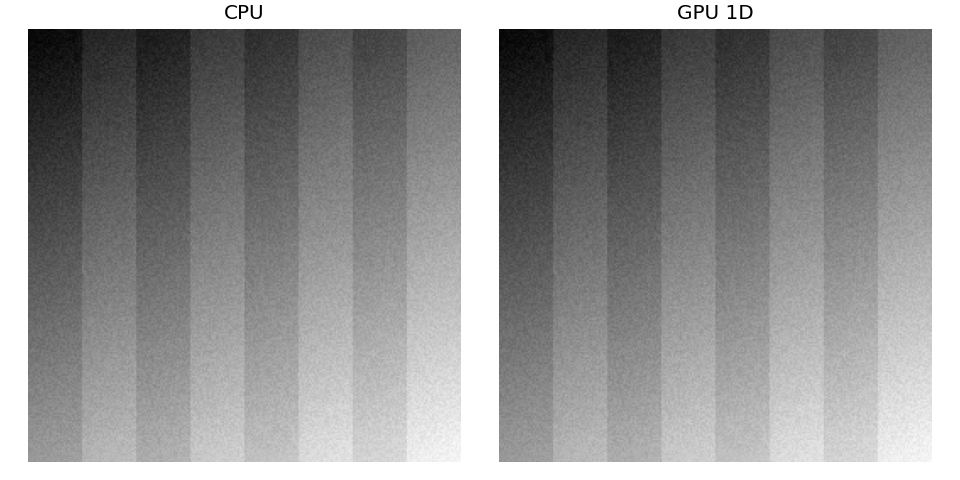
\includegraphics[width=.85\linewidth,height=.19\textheight,keepaspectratio]{figures/images.png}
\end{center}
\begin{center}
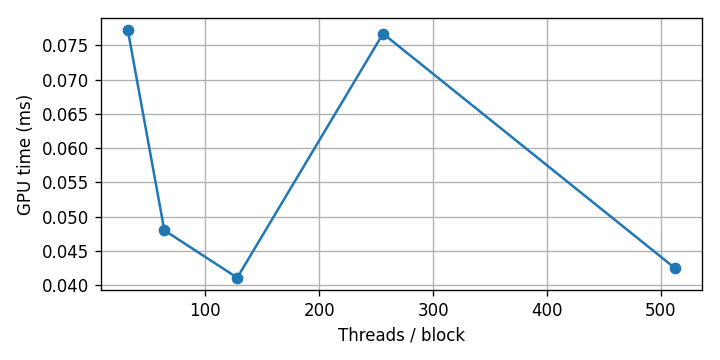
\includegraphics[width=.65\linewidth,height=.17\textheight,keepaspectratio]{figures/performance.png}
\end{center}

\section{Discussion}
The fastest measured block had 128 threads (0.0411 ms), about 10266 times faster than the Python CPU loop. The graph shows that increasing the block size does not always reduce time.

\end{document}
